\documentclass[]{article}
\usepackage[left=1in,top=1in,right=1in,bottom=1in]{geometry}


%%%% more monte %%%%
  % thispagestyle{empty}
% https://stackoverflow.com/questions/2166557/how-to-hide-the-page-number-in-latex-on-first-page-of-a-chapter
\usepackage{color}
% \usepackage[table]{xcolor} % are they using color?
  
  % \definecolor{WSU.crimson}{HTML}{981e32}
% \definecolor{WSU.gray}{HTML}{5e6a71}

% \definecolor{shadecolor}{RGB}{248,248,248}
\definecolor{WSU.crimson}{RGB}{152,30,50} % use http://colors.mshaffer.com to convert from 981e32
\definecolor{WSU.gray}{RGB}{94,106,113}

%%%%%%%%%%%%%%%%%%%%%%%%%%%%
  
  \newcommand*{\authorfont}{\fontfamily{phv}\selectfont}
    \usepackage{lmodern}
  
  
  \usepackage[T1]{fontenc}
\usepackage[utf8]{inputenc}




\usepackage{abstract}
\renewcommand{\abstractname}{}    % clear the title
\renewcommand{\absnamepos}{empty} % originally center

\renewenvironment{abstract}
{{%
  \setlength{\leftmargin}{0mm}
  \setlength{\rightmargin}{\leftmargin}%
}%
  \relax}
{\endlist}

\makeatletter
\def\@maketitle{%
  \pagestyle{empty}
  \newpage
  %  \null
  %  \vskip 2em%
    %  \begin{center}%
    \let \footnote \thanks
  {\fontsize{18}{20}\selectfont\raggedright  \setlength{\parindent}{0pt} \@title \par}%
}
%\fi
\makeatother


  
  
  
  
            
    
  
    \title{\textbf{\textcolor{WSU.crimson}{Will vs Denzel}} \newline \textbf{\textcolor{WSU.gray}{STAT 419: Final}}  }
  
  %  
  
  % \author{ \Large true \hfill \normalsize \emph{} }
\author{\Large Kathleen Rivas\vspace{0.05in} \newline\normalsize\emph{Washing=ton State University}  }
  
  
  \date{December 14, 2020}
\setcounter{secnumdepth}{3}

\usepackage{titlesec}
% See the link above: KOMA classes are not compatible with titlesec any more. Sorry.
% https://github.com/jbezos/titlesec/issues/11
\titleformat*{\section}{\bfseries}
\titleformat*{\subsection}{\bfseries\itshape}
\titleformat*{\subsubsection}{\itshape}
\titleformat*{\paragraph}{\itshape}
\titleformat*{\subparagraph}{\itshape}

% https://code.usgs.gov/usgs/norock/irvine_k/ip-092225/
  
  
  %\titleformat*{\section}{\normalsize\bfseries}
%\titleformat*{\subsection}{\normalsize\itshape}
%\titleformat*{\subsubsection}{\normalsize\itshape}
%\titleformat*{\paragraph}{\normalsize\itshape}
%\titleformat*{\subparagraph}{\normalsize\itshape}

% https://tex.stackexchange.com/questions/233866/one-column-multicol-environment#233904
\usepackage{environ}
\NewEnviron{auxmulticols}[1]{%
  \ifnum#1<2\relax% Fewer than 2 columns
  %\vspace{-\baselineskip}% Possible vertical correction
  \BODY
  \else% More than 1 column
  \begin{multicols}{#1}
    \BODY
    \end{multicols}%
    \fi
  }
  
  
  
  
  
      \usepackage{natbib}
  \setcitestyle{aysep={}} %% no year, comma just year
  % \usepackage[numbers]{natbib}
  \bibliographystyle{./../biblio/ormsv080.bst}
  
  
  
  \usepackage[strings]{underscore} % protect underscores in most circumstances
      
    
        
    
    \newtheorem{hypothesis}{Hypothesis}
  \usepackage{setspace}
  
  
  %%%%%%%%%%%%%%%%%%%%%%%%%%%%%%%%%%%%%%%%%%%%%%%%%%%%%
  %%% MONTE ADDS %%%
    
    \usepackage{fancyhdr} % fancy header 
  \usepackage{lastpage} % last page 
  
  \usepackage{multicol}
  
  
  \usepackage{etoolbox}
  \AtBeginEnvironment{quote}{\singlespacing\small}
  % https://tex.stackexchange.com/questions/325695/how-to-style-blockquote
  
  
  \usepackage{soul}			%% allows strike-through
  \usepackage{url}			%% fixes underscores in urls
  \usepackage{csquotes}		%% allows \textquote in references
  \usepackage{rotating}		%% allows table and box rotation
  \usepackage{caption}		%% customize caption information
  \usepackage{booktabs}		%% enhance table/tabular environment
  \usepackage{tabularx}		%% width attributes updates tabular
  \usepackage{enumerate}		%% special item environment
  \usepackage{enumitem}		%% special item environment
  
  \usepackage{lineno}		%% allows linenumbers for editing using \linenumbers
  \usepackage{hanging}
  
  
  \usepackage{mathtools}  	%% also loads amsmath
  \usepackage{bm}		%% bold-math
  \usepackage{scalerel}	%% scale one element (make one beta bigger font)
  
  \newcommand{\gFrac}[2]{ \genfrac{}{}{0pt}{1}{{#1}}{#2} }
    
    \newcommand{\betaSH}[3]{  \gFrac{\text{\tiny #1}}{{\text{\tiny #2}}}\hat{\beta}_{\text{#3}}   }
      \newcommand{\betaSB}[3]{              ^{\text{#1}} _{\text{#2}} \bm{\beta} _{\text{#3}}                   }  %% bold
        \newcommand{\bigEQ}{  \scaleobj{1.5}{{\ }= } }
        \newcommand{\bigP}[1]{  \scaleobj{1.5}{#1 } }
          
          
          
          
          
          \usepackage{endnotes}  % he already does this ...
          \renewcommand{\enotesize}{\normalsize}
          % https://tex.stackexchange.com/questions/99984/endnotes-do-not-be-superscript-and-add-a-space
          \renewcommand\makeenmark{\textsuperscript{[\theenmark]}} % in brackets %
            % https://tex.stackexchange.com/questions/31574/how-to-control-the-indent-in-endnotes
          \patchcmd{\enoteformat}{1.8em}{0pt}{}{}
          
          \patchcmd{\theendnotes}
          {\makeatletter}
          {\makeatletter\renewcommand\makeenmark{\textbf{[\theenmark]} }}
          {}{}
          
          
          
          % https://tex.stackexchange.com/questions/141906/configuring-footnote-position-and-spacing
          
          \addtolength{\footnotesep}{5mm} % change to 1mm
          
          \renewcommand{\thefootnote}{\textbf{\arabic{footnote}}}
          \let\footnote=\endnote
          %\renewcommand*{\theendnote}{\alph{endnote}}
          %\renewcommand{\theendnote}{\textbf{\arabic{endnote}}}
          
          
          \renewcommand*{\notesname}{}
          
          \makeatletter
          \def\enoteheading{\section*{\notesname
            \@mkboth{\MakeUppercase{\notesname}}{\MakeUppercase{\notesname}}}%
            \mbox{}\par\vskip-2.3\baselineskip\noindent\rule{.5\textwidth}{0.4pt}\par\vskip\baselineskip}
          \makeatother
          
          
          \renewcommand*{\contentsname}{}
          
          \renewcommand*{\refname}{REFERENCES}
          
          
          %\usepackage{subfigure}
          \usepackage{subcaption}
          
          \captionsetup{labelfont=bf}  % Make Table / Figure bold
          
          %%% you could add elements here ... monte says .... %%%
            %\usepackage{mypackageForCapitalH}
          
          
          %%%%%%%%%%%%%%%%%%%%%%%%%%%%%%%%%%%%%%%%%%%%%%%%%%%%%
          
          % set default figure placement to htbp
          \makeatletter
          \def\fps@figure{htbp}
          \makeatother
          
                      
            % move the hyperref stuff down here, after header-includes, to allow for - \usepackage{hyperref}
          
          \makeatletter
          \@ifpackageloaded{hyperref}{}{%
            \ifxetex
            \PassOptionsToPackage{hyphens}{url}\usepackage[setpagesize=false, % page size defined by xetex
                                                           unicode=false, % unicode breaks when used with xetex
                                                           xetex]{hyperref}
            \else
              \PassOptionsToPackage{hyphens}{url}\usepackage[draft,unicode=true]{hyperref}
            \fi
          }
          
          \@ifpackageloaded{color}{
            \PassOptionsToPackage{usenames,dvipsnames}{color}
          }{%
            \usepackage[usenames,dvipsnames]{color}
          }
          \makeatother
          \hypersetup{breaklinks=true,
          bookmarks=true,
          pdfauthor={Kathleen Rivas (Washing=ton State University)},
          pdfkeywords = {summary statistics; boxplots, normalized data, feature scaling},  
          pdftitle={Will vs Denzel: STAT 419: Final},
          colorlinks=true,
          citecolor=blue,
          urlcolor=blue,
          linkcolor=magenta,
          pdfborder={0 0 0}}
          \urlstyle{same}  % don't use monospace font for urls

% Add an option for endnotes. -----

%
% add tightlist ----------
\providecommand{\tightlist}{%
\setlength{\itemsep}{0pt}\setlength{\parskip}{0pt}}

% add some other packages ----------

% \usepackage{multicol}
% This should regulate where figures float
% See: https://tex.stackexchange.com/questions/2275/keeping-tables-figures-close-to-where-they-are-mentioned
\usepackage[section]{placeins}



\pagestyle{fancy}   
\lhead{\textcolor{WSU.crimson}{\textbf{ Will vs Denzel }}}
\chead{}
\rhead{\textcolor{WSU.gray}{\textbf{  Page\ \thepage\ of\ \protect\pageref{LastPage} }}}
\lfoot{}
\cfoot{}
\rfoot{}


\begin{document}
	
% \pagenumbering{arabic}% resets `page` counter to 1 
%
% \maketitle

{% \usefont{T1}{pnc}{m}{n}
\setlength{\parindent}{0pt}
\thispagestyle{plain}
{\fontsize{18}{20}\selectfont\raggedright 
\maketitle  % title \par  

}

{
   \vskip 13.5pt\relax \normalsize\fontsize{11}{12} 
   
\textbf{\authorfont Kathleen Rivas} \hskip 15pt \emph{\small Washing=ton State University}   

}

}








\begin{abstract}

    \hbox{\vrule height .2pt width 39.14pc}

    \vskip 8.5pt % \small 

\noindent Using data analysis, the question being asked is, ``Who is the better
actor, Will Smith or Denzel Washington?'' The answer is derived using
return on investment (ROI) and a graphing rank matrix of the top 2000
movies from the last 40 years as gathered from IMDB.


\vskip 8.5pt \noindent \textbf{\underline{Keywords}:} summary statistics; boxplots, normalized data, feature scaling \par

    




    
    \hbox{\vrule height .2pt width 39.14pc}
    \vskip 5pt 
    \hfill \textbf{\textcolor{WSU.gray}{ December 14, 2020 } }
    \vskip 5pt 
    
\end{abstract}


\vskip -8.5pt



 % removetitleabstract

\noindent  

\section{Introduction}
\label{sec:intro}

In the last 40 years, Will Smith and Denzel Washington are two of the
most prominent African-American actors in the film industry. At least
one, if not several movies of theirs shows up regularly in lists
compiled by public users on IMDB and other websites. Currently, on
Ranker, a website that uses public votes to rank a wide variety of
topics, has Denzel Washington at \#2 of 101 on the \enquote{The Best
African-American Film Actors} list. Will Smith is \#5. \citep{Ranker}

The question of \enquote{Who is the better actor?} is highly subjective
with no \enquote{right} or \enquote{one} answer. It really depends on
what is important to the person. Do film ratings determine the best? Or
how diverse the type of film which shows a willingness to experiment or
a sign of an actor less concerned with film quality? Perhaps profit
determines the best. Not only that, but what is more important -- is the
ability to potentially pull in 900\% profit once in a while better than
the ability to consistently pull in 100-200\% profit? These are not the
only \enquote{metrics} (insomuch as metrics can be applied to a
subjective subject) that can be used.

So how will I determine who is the better actor?

\section{Defining "the best"}
\label{sec:rq}

The film industry's primary reason for existence is to generate profits.
It's a business. Ratings of films, rankings, lists, movie and actor fans
woudn't exist if it wasn't profitable. Putting myself in the mind of a
film executive, my primary concern with who is the better actor is
financial. Secondary to that is the reputation of the movie -- how film
critics and the populace think how good the film is -- this would be
important for reputation contests like the Academy Awards or the Oscars.

With this in mind, the factors used for profitability analysis are
budget, usa gross, total gross. With this data, I was able to see how
much profit the movies generate, and more importantly to me, the return
on investment. Think about it. What good does generating \$900million
dollars if it took \$900 million dollars to produce? As a film
executive, this means you have gotten a 0\% return on investment --
i.e.~you broke even and made no money.

What is more important to me (if I put myself in the shoes of a film
executive), is how consistently and how large of an ROI an actor's movie
can generate for the film company. My first metric is purely profit
driven and looking at it as \enquote{two fish in a barrel}-- Will and
Denzel's profit data, side-by-side comparison.

Second in importance is how well the movie is received, and its
popularity. Popularity can help determine profit, and critical reception
is good reputation for future movies from that actor/producer/etc. Data
used for this is through a professor generated graphing rank matrix used
on the top 50 movies for each year on the last 40 years. Using the fancy
adjencency and eigenvector matrix algorithms, similar to how Google Page
Rank algorithm works for their search engine results, the MovieRank
dataset has each movie ranked (a \enquote{movieRank} number from 0-100)
within the ecosystem of the top 50 movies over the last 40 years.

Therefore, my second metric uses this larger matrix of movies as Will
and Denzel as \enquote{two fish in a pond}-- Will and Denzel's movieRank
and ROI within the larger matrix of 1,753 \enquote{top50} movies.

\subsection{Normalizing the Data}
\label{sec:rq2}

Will and Denzel's movies are ranked within the ecosystem of a larger
database of movies. However, their budget and ROI data are not (as far
as I know). Therefore, I normalized the data so that Will and Denzel's
money data is normalized within the larger movie ranking ecosystem. This
way, both movie rank and financial rank uses the same dataset and set
within the same \enquote{pool}.\\
Normalization was done on a scale of 0 to 100. To elaborate, all 1,753
movies budget and gross information was calculated to give you a sense
of how the movie did against all other movies within 0 to 100 -- people
can intuitively get a sense of the \enquote{big picture}. The larger the
number, the \enquote{better} the score or rank. The formula used:

\begin{equation}
\label{eq:my-formula}
    X^{scaled} = \frac{X_i}{\sum_{i=1}^{\infty} X_{i}}  
\end{equation}

\section{Data Description}
\label{sec:data}

The size of this ecosystem is 1,998 movies. With all the NAs removed
from budget and global gross columns, I ended up with 1,753 movies. The
dataset was provided for me by the professor who used a graph rank
matrix algorithm to calculate \enquote{movieRank}.

I calculated ROI for each movie, both on US profit, and total profit
(worldwide and US combined). Then, I normalized three features --
budget, ROI on US only, and ROI Total.

From this dataset, I then extracted the Will and Denzel's movies. Each
had 19 movies appear in an IMDB top 50 list over the course of 40 years.
This was further reduced to 17 movies each for comparison. Some movies
were removed due to lack of financial information (Ma Rainey's Black
Bottom (2020) {[}Denzel{]} and Fallen (1998) {[}Denzel{]}). One movie
was removed due to an error -- Will Smith was tagged with Austin Powers:
The Spy Who Shagged Me (1999), but did not appear in the cast credits on
the IMDB webpage. A William Smith is in the credits, but not as an
actor. I removed it from Will Smith's list of top movies, but kept the
movie information within the larger dataset for normalization reasons.

The top movies that Will and Denzel made that were analyzed are as
follows:

\vspace{10mm}
\begin{tabular}{c c}
  Will Smith & Denzel Washington \\
  \hline
  Independence Day (1996) & The Pelican Brief (1993) \\
  Enemy of the State (1998) & American Gangster (2007) \\
  Men in Black (1997) & Glory (1989) \\
  Men in Black II (2002) & Training Day (2001) \\
  Men in Black 3 (2012) & Inside Man (2006) \\
  Bad Boys II (2003) & Deja Vu (2006) \\
  Wild Wild West (1999) & The Book of Eli (2010) \\
  I, Robot (2004) & Much Ado About Nothing (1993) \\
  Hancock (2008) & The Magnificent Seven (2016) \\
  Suicide Squad (2016) & Crimson Tide (1995) \\
  Hitch (2005) & Man on Fire (2004) \\
  The Pursuit of Happyness (2006) & Remember the Titans (2000) \\
  Focus (2015) & Philadelphia (1993) \\
  Bad Boys (1995) & The Equalizer (2014) \\
  I am Legend (2007) & The Equalizer 2 (2018) \\
  Aladdin (2019) & Malcolm X (1992) \\
  The Karate Kid (2010) & Flight (2012) 
  
\end{tabular}

\subsection{Summary of Will and Denzel}
\label{sec:data-sample}

In order to understand Will and Denzel's movies in context to the larger
\enquote{pool} of movies, understanding Will and Denzel's individual
data comes first. In order to do that, here is an overview of Will and
Denzel's movies:

The total number of movies Will has made: 48 The total number of movies
Denzel has made: 40 Note: I removed many pre-production and possible
productions from the datasets. (Will had a large amount of these.)
\vspace{5mm} Summary Statistics on the Return on Investment:
\vspace{5mm} Will Smith

\vspace{5mm}
\begin{tabular} {c c c c c c c}
  Min & Q1 & Median & Mean & Q3 & Max & NA's \\
  \hline
  -81.05\% & 22.66\% & 177.35\% & 221.21\% & 323.20\% & 989.87\% & 5
\end {tabular}
\vspace{5mm}

Denzel Washington

\vspace{5mm}
\begin{tabular}{c c c c c c c}
  Min & Q1 & Median & Mean & Q3 & Max & NA's \\
  \hline
  -79.66\% & 48.41\% & 99.10\% & 129.58\% & 180.45\% & 694.92\% & 2
\end{tabular}

\vspace{5mm}

In exploring the datasets, I thought of several questions related to
money. I noticed that there were many instances where the movies lost
money in the US, yet still managed to profit in total due to the
worldwide sales. It showed me, data-wise, how important the global
market is in the film industry.

As an aside, this made me wonder if the recent push towards
\enquote{diversity} is less altruistic and more financially driven --
Matt Damon's participation in The Great Wall (2017) and the recent
influx of Asian-American based content (such as Crazy Rich Asians
(2018)). The Internet has really made global content easily flexible
which has caused interesting shifts such as the influence of K-pop
through YouTube, etc. It makes sense to create content that would appeal
to this demographic, albeit in a more niche sort of fashion.
\vspace{5mm}

For the following summary statistics, due to NA's, Will's total movies
analyzed are 43 and Denzel's are 38.

In any case, how many times did the global market save a movie from US
profit loss?\\
\vspace{5mm} For Will, that is 9 times out of 14 (64.29\%). 17/43 movies
did not break even in the US, yet only 8 movies out of that did not
break even total. However, three of those were not globally distributed,
so out of 14 movies, the global market made enough to break even or more
9 times.

For Denzel, that is once (100\%). Out of 6 movies that lost profit
total, only 1 of these 6 profit-loss movies were distributed globally
and lost. This sounds like Denzel loses more profit than Will, but that
is not the case. \vspace{5mm} Movies that did not break even in the US:
Will: 17/43 (47.1\%) Denzel: 13/38 (34.21\%)

Movies that did not break even total: Will: 9/43 (20.93\%) Denzel: 6/38
(15.79\%)

Movies that made more than (an arbitrary) \$50 million in profit: Will:
25/43 (58.14\%) Denzel: 20/38 (52.63\%) \vspace{5mm} At this point, I am
not sure who is the better actor. In a sense, what type of film
executive am I? Am I the type of person who wants a consistent US profit
only type of profit? Am I the type that wants to make as much profit as
I can in the long run (i.e.~with global profits)?

If I was only interested in consistency, Denzel is the better actor. His
percent to return has a lower minimum loss, a better Q1 than Will. He
will generally lose less money than Will will. However, if I was
interested in the greater profits, Will is the better actor -- his
median score is better than Denzel's, and his upper range at Q3 and Max
exceed Denzel's by 142.75\% and 294.95\% times.

\subsection{Summary Statistics of Data}
\label{sec:data-summary}

Looking at Will and Denzel as \enquote{two fish in a barrel} provided
some perspective on their individual ROI performance. Will's potential
range is wider than Denzel's -- he not only can generate greater ROI,
but also lower ROI.

However, critical reception is also another metric important to a film
executive. There is prestige when a movie wins Best Picture at the
Oscars or other film competitions. There may be long term profits
associated with films that have attained Best Picture.

The following is a summary table, a side by side comparison of the
movies that have made it to the top50 lists, and where it ranks within
the larger dataset of movieRank.

\vspace{5mm}

\hspace*{-2cm}\begin{tabular}{|c c c |c c c| }
\hline
Will's Movies & Movie Rank & ROI Rank & ROI Rank & Movie Rank & Denzel's Movies \\
\hline
  
Independence Day (1996) & 47.49 & .077 & .011 & 58.66 & The Pelican Brief (1993) \\
Enemy of the State (1998) & 43.02 & .014 & .006 & 48.04 & American Gangster (2007) \\
Men in Black (1997) & 41.9 & .043 & .007 &  44.69 & Glory (1989) \\
Men in Black II (2002) & 41.34 & .017 & .007 & 43.58 & Training Day (2001) \\
Men in Black 3 (2012) & 40.78 & .014 & .013 & 43.58 & Inside Man (2006) \\
Bad Boys II (2003) & 34.64 & .009 & .004 & 39.66 & Deja Vu (2006) \\
Wild Wild West (1999) & 34.08 & .002 & .004 & 39.11 & The Book of Eli (2010) \\
I, Robot (2004) & 34.08 & .015 & .016 & 37.99 & Much Ado About Nothing (1993) \\
Hancock (2008) & 32.96 & .025 & .01 & 37.99 & The Magnificent Seven (2016) \\
Suicide Squad (2016) & 24.02 & .025 & .015 & 37.43 & Crimson Tide (1995) \\
Hitch (2005) & 22.35 & .033 & .019 & 35.2 & Man on Fire (2004) \\
The Pursuit of Happyness (2006) & 21.79 & .036 & .024 & 29.05 & Remember the Titans (2000) \\
Focus (2015) & 20.11 & .017 & .008 & 27.37 & Philadelphia (1993) \\
Bad Boys (1995) & 16.2 & .05 & .03 & 26.82 & The Equalizer (2014) \\
I am Legend (2007) & 12.85 & .023 & .054 & 20.67 & The Equalizer 2 (2018) \\
Aladdin (2019) & 12.85 & .037 & .033 & 20.11 & Malcolm X (1992) \\
The Karate Kid (2010) & 6.15 & .062 & .028 & 17.32 & Flight (2012) \\
\hline
\end{tabular}
\vspace{5mm}

The key takeaway from this table is that you can see that Will's movies
score higher in ROI rank. Inversely so, Denzel's movies all have a
higher movieRank score than Will's.

Keep in mind that the scaled ROI had two extreme outliers -- Paranormal
Activity (2007) (ROI Rank: 100) and The Blair Witch Project (1999) (ROI
Rank: 32.14). The third highest rank after these two is Clerks (1994)
(ROI Rank: .89). It drops from 32.14 to .89! And subsequently lower down
to the negatives (those that have lost money). So that needs to be kept
in mind when looking at Will and Denzel's ROI rankings.

The movieRank scale is more evenly dispersed throughout so it's easier
for the human brain to comprehend those movie rankings of
\enquote{24.02(\%)} than \enquote{.036(\%)}.

\section{Key Findings}
\label{sec:findings}

So, my original premise was to create a type of indexed score that would
represent both of these ranks by multiplying movieRank and ROI rank
together. Then, I would evaluate this score, discuss the findings, and
then construct a visualization of this indexed score. This indexed
score, in a side by side comparison resulted in Will's \enquote{win}. (9
Will wins and 8 Denzel losses)

I've counted the above summary table multiple ways. I've multiplied
actorRank, movieRank, and ROI rank -- Denzel wins in this case, because
his higher actorRank score (35.99 vs Will's 32.01) helps boost his lower
ROI score. I thought this was an unfair advantage of Denzel's because
actor Rank is pretty subjective. So I removed actorRank from the
scoring. I've also tried multiplying movieRank and their individual ROIs
(instead of ROI rank), and while they may have adjusted the
\enquote{wins and losses} a little, Will still \enquote{won}.

The only time (other than using actorRank) that Denzel \enquote{won} was
when I would tally who had the higher score, irrespective by how much
higher. For example, if Will's movie 1 had a higher movieRank, he would
get a 1, if Will's ROI was higher, another tally to 2, and a third
metric was used in this case as a \enquote{tie-breaker}, the ROI on US
profits alone (the modern Hollywood strategy to break even in the US box
office and profit in the world box office). If Will's movie 1 had a
lower score than Denzel's movie 1, then the final score for the first
side by side comparison was Will:2, Denzel:1 -- Will wins the first
round. And so on and so forth.

With this method, Denzel won.

But I decided that this wouldn't be fair to Will's range of profit
potential. Can Denzel's ROI of 333.929\% for The Pelican Brief to Will's
Independence Day ROI of 989.868\% really be compared equally to Denzel's
ROI of 207.097\% for The Equalizer 2 to Will's ROI of 290.273\% for I Am
Legend? The difference between the first is huge, and the second is
quite close.

The same would go for movieRank differences.

However, during my data analysis journey, I came across webpages that
decried the use of an indexed score, saying that it reduced the
complexity of a multivariate system and provided an oft-misleading
convenient single number. \citep{StackExchange} And I am torn. Because
when I read these opinions, intuitively I agree. But a single number
would be convenient since my summary table of Will and Denzel's top
movies ranked with the larger \enquote{pond} has opposite results --
Denzel's movieRank is higher, and Will's ROI rank is higher, across the
board. Combining the score allows me to rank them more conveniently.

The following is a visualization of three boxplots. The first is the
boxplot of the \enquote{pond} ROI rank scores. This is to provide
context to the following boxplots -- Will's and Denzel's ROI rank
scores. I did remove the two extreme outliers (Paranormal Activity and
The Blair Witch Project) because they distorted the visualization too
much to read Will's and Denzel's boxplots. Even with the outliers
removed, Will and Denzel's ROI rank boxplots are small in perspective to
the \enquote{pond}.

\begin{center}
        \scalebox{1.00}{    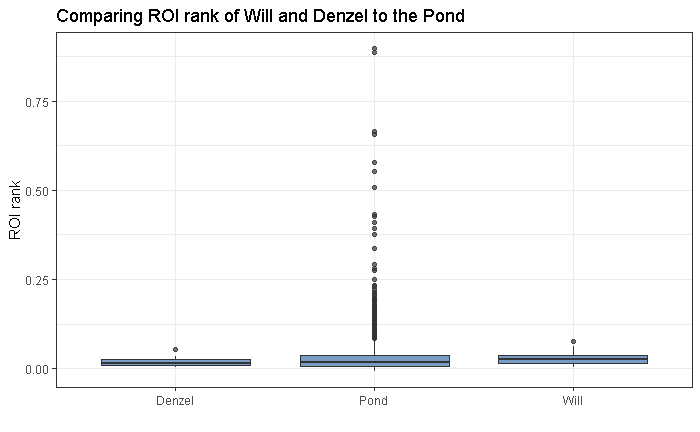
\includegraphics[trim = 0 0 0 0,clip,width=\textwidth]{figures/boxplot.png} }
    \end{center}

\label{fig:Boxplot}

If you look closely at the boxplot, you will see that the median ROI
rank for Will is higher than the median ROI rank of \enquote{the Pond}
and the median ROI rank score for Denzel is lower than \enquote{the
Pond's}.

In the end, I define \enquote{the best} as the one with the better ROI.
The \enquote{best} actor is the one who had a higher ROI. The movieRank
was placed as a secondary consideration. An \enquote{indexed} score
would help but not looked upon favorably but not necessary. When placing
Will's and Denzel's ROI rank within the framework of the
\enquote{pond's} ROI rank, it is clear that Will's ROI is higher than
Denzel's.

\section{Conclusion}
\label{sec:conclusion}

While Denzel's high movieRank scores mitigate his lower ROI rank score,
it is not enough to overcome Will's higher ROI rank scores. The data
analysis of the ROI of the two actors, as well as how they do compared
to many movies within the same time period shows this. As an imaginary
film executive, I would pick Will Smith to be the actor over Denzel
Washington.

However, movies are not created in isolation. It is a vast machinery,
with many components. Even just focusing on ROI alone can be
complicated. There are many interesting layers to answering this
question that did not get explored. If there were a way to include
actorRank, and the actorRanks of their co-stars, would be interesting.
The popularity of other actors (and directors) play a part in the
success of a film. I also wanted to look into profitability of movies
over time. Perhaps Denzel's \enquote{star power} is fading over the
years. Or perhaps Will's. When is their \enquote{peak} profitability or
perhaps it's a uniform distribution.




%% appendices go here!


\newpage
\theendnotes

%%%%%%%%%%%%%%%%%%%%%%%%%%%%%%%%%%%  biblio %%%%%%%%
\newpage
\begin{auxmulticols}{1}
\singlespacing 
\bibliography{./../biblio/master.bib}

%%%%%%%%%%%%%%%%%%%%%%%%%%%%%%%%%%%  biblio %%%%%%%%
\end{auxmulticols}

\newpage
{
\hypersetup{linkcolor=black}
\setcounter{tocdepth}{3}
\tableofcontents
}



\end{document}